\setchapterpreamble[u]{\margintoc}
\chapter[Rotation of the quadrupole tensor around the z-axis]{Rotation of the quadrupole tensor around the $z$-axis}
\label{app:rotations_quadrupole}

We start from the Cartesian, symmetric traceless tensor

\begin{equation}
Q=\begin{pmatrix}
Q_{xx} & Q_{xy} & Q_{xz}\\
Q_{xy} & Q_{yy} & Q_{yz}\\
Q_{xz} & Q_{yz} & Q_{zz}
\end{pmatrix},\qquad \mathrm{Tr}\,Q=0,
\end{equation}

and rotate the axes by an angle $\phi$ about $z$ with

\begin{equation}
R_z(\phi)=
\begin{pmatrix}
\cos\phi & \sin\phi & 0\\
-\sin\phi & \cos\phi & 0\\
0 & 0 & 1
\end{pmatrix}.
\end{equation}
Under this passive rotation,
\begin{equation}
Q' \;=\; R_z(\phi)\,Q\,R_z^\top(\phi).
\end{equation}

Carrying out the multiplication gives

\begin{equation}
\begin{aligned}
Q'_{xx} &= \cos^2\!\phi\,Q_{xx}+\sin^2\!\phi\,Q_{yy}+2\sin\phi\cos\phi\,Q_{xy},\\
Q'_{yy} &= \sin^2\!\phi\,Q_{xx}+\cos^2\!\phi\,Q_{yy}-2\sin\phi\cos\phi\,Q_{xy},\\
Q'_{xy} &= (\cos^2\!\phi-\sin^2\!\phi)\,Q_{xy}+\sin\phi\cos\phi\,(Q_{yy}-Q_{xx}),\\
Q'_{xz} &= \cos\phi\,Q_{xz}+\sin\phi\,Q_{yz},\\
Q'_{yz} &= -\sin\phi\,Q_{xz}+\cos\phi\,Q_{yz},\\
Q'_{zz} &= Q_{zz}.
\end{aligned}
\label{eq:Qprime-cart}
\end{equation}

We define the spherical components (rank-2 irreducible combinations) as

\begin{equation}
\begin{aligned}
S_0 &= Q_{zz},\\
S_{\pm1} &= Q_{xz}\pm iQ_{yz},\\
S_{\pm2} &= \tfrac12\,(Q_{xx}-Q_{yy}) \pm i\,Q_{xy}.
\end{aligned}
\label{eq:Q-spherical-def}
\end{equation}

Using \ref{eq:Qprime-cart} in the definition of $S'_{\pm1}$,

\begin{equation}
\begin{aligned}
S'_{+1}
&= Q'_{xz}+i\,Q'_{yz}\\
&= \big(\cos\phi\,Q_{xz}+\sin\phi\,Q_{yz}\big)\;+\;i\big(-\sin\phi\,Q_{xz}+\cos\phi\,Q_{yz}\big)\\
&= (\cos\phi - i\sin\phi)\,Q_{xz}\;+\;(\sin\phi + i\cos\phi)\,Q_{yz} =\; e^{-i\phi}\,S_{+1}.
\end{aligned}
\end{equation}

Similarly,

\begin{equation}
\begin{aligned}
S'_{-1}
&= Q'_{xz}-i\,Q'_{yz}\\
&= \big(\cos\phi\,Q_{xz}+\sin\phi\,Q_{yz}\big)\;-\;i\big(-\sin\phi\,Q_{xz}+\cos\phi\,Q_{yz}\big)\\
&= (\cos\phi + i\sin\phi)\,Q_{xz}\;+\;(\sin\phi - i\cos\phi)\,Q_{yz}\\
&= e^{+i\phi}\,\big(Q_{xz}-iQ_{yz}\big) \;=\; e^{+i\phi}\,S_{-1}.
\end{aligned}
\end{equation}

Let $\Delta Q \equiv Q_{xx}-Q_{yy}$. From \eqref{eq:Qprime-cart},

\begin{equation}
\begin{aligned}
S'_{+2}
&= \tfrac12\,(Q'_{xx}-Q'_{yy}) + i\,Q'_{xy}\\
&= \tfrac12\Big[\big(\cos^2\!\phi-\sin^2\!\phi\big)\Delta Q  + 4\sin\phi\cos\phi\,Q_{xy}\Big]\\
&+ i\Big[\big(\cos^2\!\phi-\sin^2\!\phi\big)Q_{xy} - \sin\phi\cos\phi\,\Delta Q \Big].
\end{aligned}
\end{equation}

Use the double-angle identities $\cos 2\phi=\cos^2\!\phi-\sin^2\!\phi$ and $\sin 2\phi=2\sin\phi\cos\phi$ to rewrite
\begin{equation}
\begin{aligned}
S'_{+2}
&= \tfrac12\Big[\cos 2\phi\,\Delta Q  + 2\sin 2\phi\,Q_{xy}\Big]
+ i\Big[\cos 2\phi\,Q_{xy} - \tfrac12\sin 2\phi\,\Delta Q \Big]\\[4pt]
&= \left(\tfrac12\Delta Q  + iQ_{xy}\right)\big(\cos 2\phi - i\sin 2\phi\big)\\[4pt]
&= \left(\tfrac12\Delta Q  + iQ_{xy}\right) e^{-i2\phi}
\;=\; e^{-i2\phi}\,S_{+2}.
\end{aligned}
\end{equation}

By complex conjugation or repeating the steps with $-i$,

\begin{equation}
S'_{-2} \;=\; e^{+i2\phi}\,S_{-2}.
\end{equation}

Since $Q'_{zz}=Q_{zz}$,
\begin{equation}
S'_0 \;=\; S_0.
\end{equation}

Collecting the results,

\begin{equation}
S'_m \;=\; e^{-im\phi}\,S_m,\qquad m=0,\pm1,\pm2.
\end{equation}


\chapter{Single Microwave Photon Detector}
\label{app:SMPD}

The detection of single optical photons is performed routinely via photomultipliers and superconducting nanowire photon detectors. However, microwaves are five orders of magnitude less energetic than optical photons, and single-photon detection is not trivial. Our group proposed and developed a detector based on a superconducting circuit with a transmon qubit at its center~\sidecite{lescanne_irreversible_2020}. In the following, we describe the SMPD architecture, its operating principle, and the key performance metrics (efficiency, dark-count rate, and temporal resolution) relevant for detecting microwave fluorescence from individual \Er ions. For an in-depth description and characterization of the SMPD, one should refer to previous theses from the group, which focus on the development and fabrication of this device, particularly \cite{albertinale_detecting_2021,balembois_magnetic_2023,pallegoix_high_2025}.

\section{Working principle}

The operating principle of the SMPD can be summarized as follows: an incoming photon is detected by performing an irreversible frequency conversion into a qubit excitation. After the detection window, the qubit is read out dispersively, revealing the arrival of the photon. The architecture is based on the irreversibility of the process, enabled by an engineered dissipation mechanism.

\begin{marginfigure}
    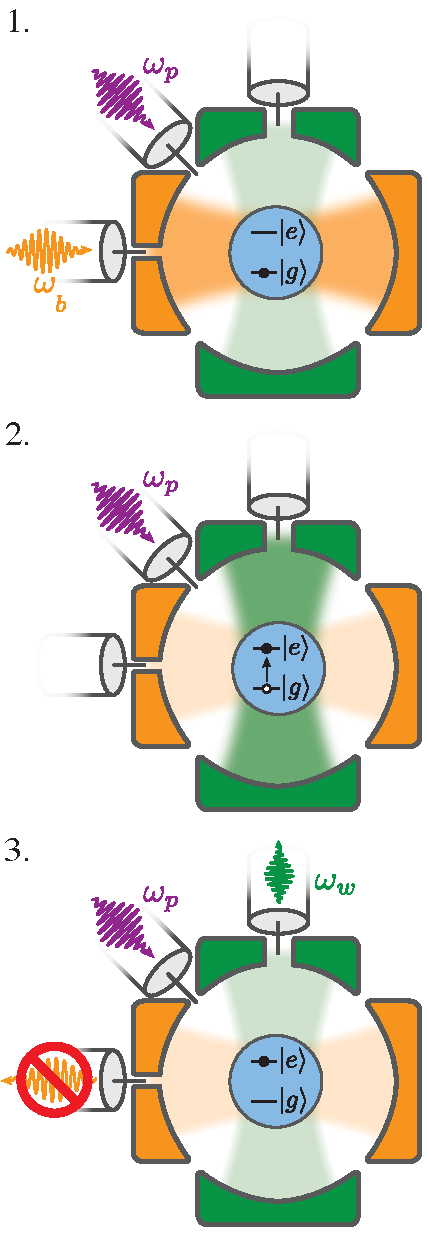
\includegraphics{chapter2/figures/SMPD_principle.pdf}
    \caption[SMPD working principle]{Working principle of the SMPD. At the heart of the SMPD lies a qubit with states $\ket{g}$ and $\ket{e}$. There are two resonators coupled to the qubit, the buffer and the waste in orange and green respectively, as well as a transmission line to drive and pump the qubit. The capturing process is divided in three steps. First, capture of the incoming photon. Second, four-wave mixing, where the buffer photon is transformed into a qubit excitation. Third, dissipation of the waste, which inhibits the reverse process.}
    \labfig{SMPD_principle}
\end{marginfigure}

At the center of the SMPD lies a superconducting transmon qubit\sidecite{koch_chargeinsensitive_2007}. This element behaves as a nonlinear oscillator and can be treated as an effective two-level system with frequency $\omega_q$ and levels $\ket{g}$ and $\ket{e}$. The qubit is simultaneously coupled to two independent resonators: the \textit{buffer} resonator with frequency $\omega_b$ and the \textit{waste} resonator with frequency $\omega_w$. The process that enables the frequency conversion is a parametric four-wave mixing (4WM), in which a buffer photon is mixed with a coherent pump tone to produce an excitation on the qubit and a waste photon. The detection process is divided into two distinct phases: the capture phase, when the qubit excitation via 4WM takes place, and the readout phase, when the state of the qubit is measured.

The capturing process can be summarized in three independent steps which are schematized in \reffig{SMPD_principle}.

\begin{enumerate}
    \item A photon traveling in the microwave lines with frequency $\omega_b$ arrives at the input of the detector, populating the buffer resonator. Meanwhile, the SMPD is illuminated with a coherent pump tone at frequency $\omega_p$.
    \item With the input resonator populated, the 4WM process transforms the buffer photon and a pump photon into a qubit excitation and a waste photon. 
    \item To avoid the inverse process, a dissipation channel on the waste resonator is engineered by strongly coupling it to the microwave lines. Consequently, the waste photon is rapidly lost (hence the name), blocking the reverse parametric process from ever taking place.
\end{enumerate}

It is important to note that, for the 4WM process to take place, energy conservation must be satisfied:

\begin{equation}
    \omega_b + \omega_p = \omega_q + \omega_w,
\end{equation}

This relation can be ensured by adjusting the frequency of the pump tone.

After the capturing process, the state of the qubit is read out dispersively using a coherent tone on the waste resonator \sidecite{wallraff_strong_2004}. If the qubit is found in the ground state, the detection cycle can restart. However, if the qubit is in the excited state, it first needs to be reset to the ground state before restarting the capturing phase. One could just wait for the qubit to spontaneously relax, but the detector is not operational during this process, effectively reducing the detection efficiency. We implement a conditional reset, in which a $\pi$-pulse is applied if the qubit is found in the excited state, followed by another readout step. This repeats until the qubit is in its ground state. Thanks to the high fidelity of the excited-state readout, this procedure also effectively cools down the qubit. The detection process is performed continuously in cycles and can be visualized in \reffig{SMPD_cycle}. We define the capture, readout, and reset times as $\tau_\text{capture}$, $\tau_\text{ro}$, and $\tau_\text{reset}$, respectively.

\begin{figure}
    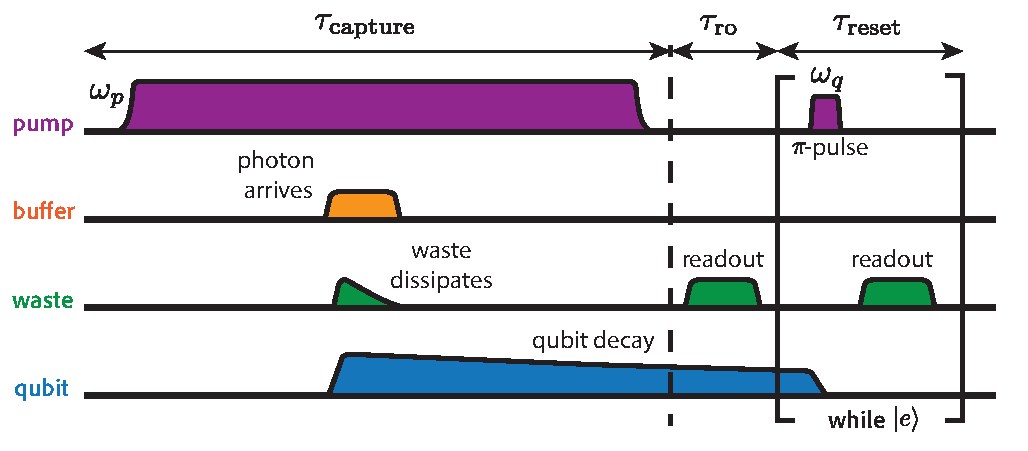
\includegraphics{chapter2/figures/SMPD_cycle.pdf}
    \caption[SMPD cycle]{The SMPD cycle is divided into two parts, the capture and readout phases, separated by a dashed line. During the detection phase, the pump tone at frequency $\omega_p$ illuminates the qubit continuously. An incoming photon triggers 4WM and the qubit is excited while the waste photon is rapidly dissipated. During the readout phase, the qubit is measured using the dispersive shift of the waste resonator. If the qubit is excited, a $\pi$-pulse is applied through the pump line at frequency $\omega_q$, then the qubit is read out again until it is found in the ground state.}
    \labfig{SMPD_cycle}
\end{figure}

We note that only photons that arrive during the capturing phase will be detected, as the 4WM process is turned off during the readout phase. In addition, if a second photon arrives at the detector, the 4WM process will not take place, as the qubit is already in the excited state. Consequently, if the input photon rate exceeds the SMPD cycle rate, the detector will saturate and is effectively "blinded".

\section{SMPD Circuit}

\begin{figure*}
    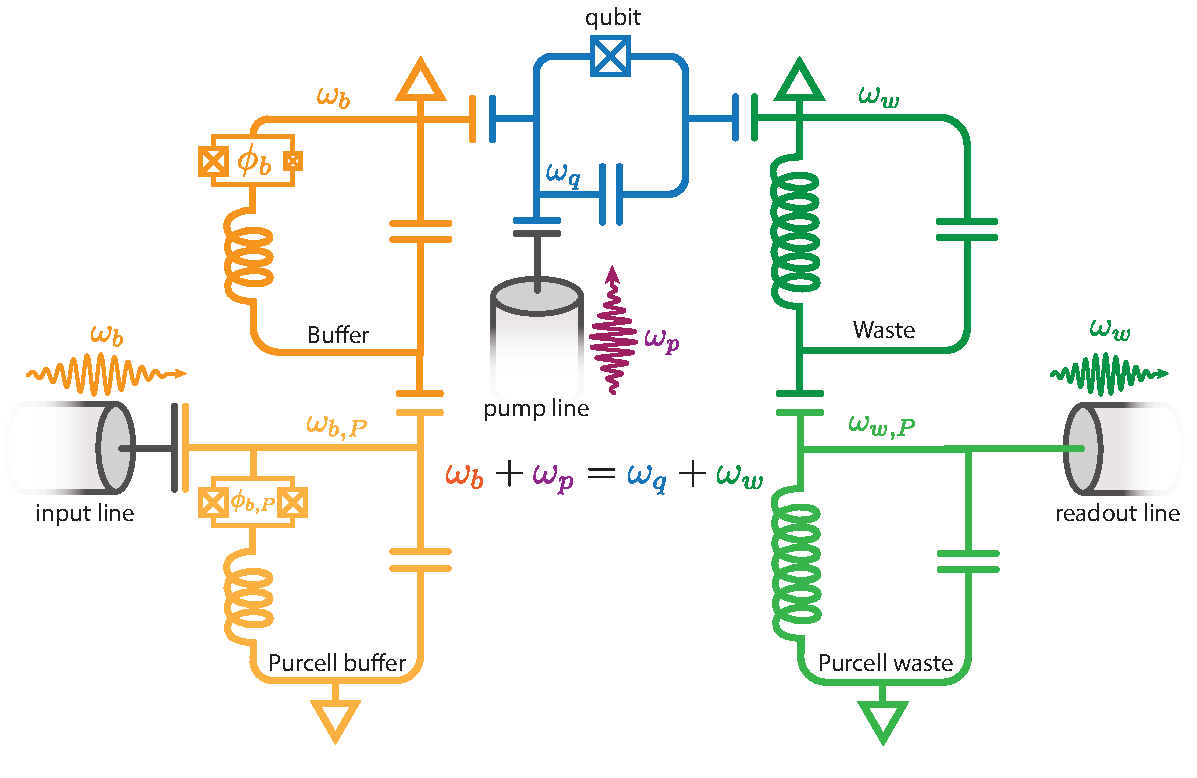
\includegraphics{chapter2/figures/SMPD.pdf}
    \caption[SMPD circuit]{SMPD schematic circuit. The qubit (blue) has a fixed frequency and is capacitively coupled to both the waste and the buffer resonators. Both the buffer and its Purcell filter (dark and light orange, respectively) embed a SQUID, used to tune their frequencies. The SQUID of the buffer is strongly asymmetric to reduce spectral diffusion due to magnetic noise. The buffer Purcell filter is capacitively coupled to the input microwave line. The waste and its Purcell filter have a fixed frequency. In contrast to the buffer's, the waste Purcell filter is galvanically coupled to the output microwave line, which ensures a rapid dissipation of any waste photon. The qubit is also capacitively coupled to a CPW line, used to pump the 4WM process and coherently control its state.}
    \labfig{SMPD_circuit}
\end{figure*}

We now proceed to describe the individual components of the SMPD. The device is fabricated from a tantalum thin film on a sapphire chip using standard nanofabrication techniques and all Josephson junctions are made from a tri-layer of Al/AlO$_x$/Al \sidecite{pallegoix_high_2025}. \reffig{SMPD_circuit} shows a schematic representation of the circuit. 

\begin{itemize}
    \item \textbf{Qubit.} Transmon design with a Josephson junction and shunted capacitor. It is dispersively coupled to both buffer and waste resonators. For robustness, the frequency of the qubit is non-tunable.
    \item \textbf{Buffer.} The buffer resonator is the capture port for incoming photons. It takes the form of a half-wave coplanar waveguide (CPW) with open ends. One end couples capacitively to the qubit. The resonator has a SQUID embedded in its design \sidenote{A Superconducting Quantum Interference Device (SQUID) is a non-linear element with a tunable inductance. It is composed of two Josephson junctions in parallel, forming a loop. The magnetic flux threading the loop modulates periodically the inductance of the element. Experimentally, the flux is controlled by means of a DC current that runs on a nearby grounded line, which generates a local magnetic field.}. The SQUID is highly asymmetric to reduce spectral diffusion of the buffer resonator.
    \item \textbf{Buffer Purcell filter.} The middle of the buffer resonator is capacitively coupled to the buffer Purcell filter. This second resonator prevents the qubit from rapidly decaying to the microwave lines due to its interaction with the buffer. Additionally, the Purcell filter embeds a SQUID element in the middle of its design. By tuning the frequency of the Purcell filter, the effective detection bandwidth can also be controlled.
    \item \textbf{Waste and its Purcell filter.} The waste resonator receives the converted photon produced by the four-wave mixing process and is also used for dispersive readout. It is galvanically coupled to the microwave lines so that the waste photon is rapidly lost, and the conversion becomes effectively irreversible. The Purcell filter is designed with the same principle as the buffer's.
    \item \textbf{Qubit drive line.} The dedicated pump line delivers the coherent pump tone at $\omega_p$ used for 4WM as well as controlling the state of the qubit. The line is designed as a simple CPW element capacitively coupled to the qubit.
\end{itemize}

All relevant frequencies and linewidths of the elements from the SMPD used in this work are displayed in \reftab{SMPD_frequencies}. 

\begin{table}[h!]
\centering
\begin{tabular}{|l|c|c|}
\hline
\textbf{Resonator} & \textbf{Frequency} (GHz) & \textbf{Linewidth} (MHz) \\ \hline
Buffer & $\omega_{b}/2\pi \in [7.70;7.76]$ & $\sim[0;2.5]$ \\ \hline
Buffer Purcell & $\omega_{b, P}/2\pi \in [7.26;7.78]$ & 20 \\ \hline
Qubit & $\omega_{q}/2\pi = 6.533$ & 0.016 \\ \hline
Waste & $\omega_{w}/2\pi = 8.475$ & 1.75 \\ \hline
Waste Purcell & $\omega_{w, P}/2\pi \approx 8.39$ & 400 \\ \hline
\end{tabular}
\caption[SMPD frequencies]{Frequencies and linewidths of different elements of the SMPD. The linewidth of the buffer is controlled by tuning the frequency of the buffer's Purcell filter. The data was taken from \cite{pallegoix_enhancing_2025}.}
\labtab{SMPD_frequencies}
\end{table}

\section{Performance metrics}

To characterize the detector, we define a series of performance metrics, namely the efficiency, the dark-count rate, and the bandwidth of the detector. We now proceed to discuss each of them and how they relate to the performance of the detector.

\paragraph{Efficiency}

We define the efficiency $\eta_\text{SMPD}$ as the probability of successfully detecting a photon arriving at the detector. There are numerous sources of detection infidelity:

\begin{itemize}
    \item \textbf{Conversion efficiency}. The 4WM process is not instantaneous; it is a coherent process with an associated rate. Given the finite losses of the buffer resonator, some photons will inevitably be lost during the conversion process. The efficiency of the process can be estimated as \sidenote{Here we assume that the cooperativity of the parametric process is equal to 1. A more detailed study of the 4WM process is outside the scope of this thesis and can be found in \cite{pallegoix_high_2025}} \[\eta_\text{b, loss} = \frac{1}{1 + \tfrac{\kappa_\text{b, i}}{\kappa_\text{b, c}}},\] where we separate the losses of the buffer between internal ($\kappa_\text{b, i}$) and coupling ($\kappa_\text{b, c}$) contributions.
    
    \item \textbf{Duty cycle}. During the readout phase of the detector, the parametric conversion is turned off. This interval defines the dead time of the detector. The efficiency associated with the dead time can be estimated by \[\eta_\text{dead} = \frac{\tau_\text{capture}}{\tau_\text{capture} + \tau_\text{ro}},\] where we have assumed that the reset time is negligible due to the low photon arrival rate. This can be maximized by extending the capture time with respect to the readout time.
    
    \item \textbf{Qubit lifetime}. Given the finite lifetime of the qubit, $T_{1, q}\approx80$~\textmu s, any excitation will eventually be lost. The efficiency associated with this loss channel is given by averaging the loss probability over the detection window, \[\eta_{q} = \frac{1}{\tau_\text{capture}}\int_0^{\tau_\text{capture}} e^{-(\tau_\text{capture} - t)/T_1}dt = \frac{T_1}{\tau_\text{capture}} \left(1 -e^{-\tau_\text{capture}/T_1} \right) \] Assuming that $\tau_\text{capture}\ll T_1$, we arrive at \[\eta_{q}\approx 1 - \frac{\tau_\text{capture}}{2T_1},\] From this expression, we conclude that a short detection window compared to the decay time of the qubit minimizes losses in the qubit.
    
    \item \textbf{Measurement efficiency}. After the conversion, the qubit is read out dispersively. The measurement has a finite fidelity $\eta_\text{q, meas}$, which increases with the qubit readout time. In our experiments, the single-shot threshold is chosen to minimize false positives (dark counts) at the expense of increased false negatives. This choice is made due to the low number of arriving photons; a large false positive rate would disproportionately corrupt the measurement statistics.
  
\end{itemize}

The total efficiency of the detector is obtained by combining all sources of infidelity

\begin{equation}
    \eta_\text{SMPD} = \eta_{b, \text{loss}} \times \eta_\text{dead} \times \eta_{q} \times \eta_{q, \text{meas}}
\end{equation}

We can see that there are conflicting requirements to maximize both $\eta_{q}$ and $\eta_\text{dead}$. Extending the detection window increases $\eta_\text{dead}$ while reducing $\eta_q$, and a compromise must be made. In addition, increasing the readout time to achieve a high readout fidelity effectively increases the dead time of the detector. In the end, we set the detection window and the readout time to $\tau_\text{capture}=17$~\textmu s and $\tau_\text{ro}=1$~\textmu s, from which we estimate $\eta_\text{dead}=0.94$ and $\eta_{q}=0.90$. We choose a single-shot threshold that heavily suppresses false positives, with $P(e|g)\approx2\times10^{-3}$, which is close to the optimal condition.

\paragraph{Dark counts} 

The dark count rate of the detector $\Gamma_\text{DC}$ is defined as the detection rate when the device is operated without any input signal. As we approach unity efficiency, dark counts become the limiting factor on the detection sensitivity, and a large effort in the group is directed toward minimizing them \sidecite{may_noise_2025}. The origin of the dark counts can be traced back to two main effects: spurious qubit excitations and thermal photons on the microwave lines.

Given that the experiments are performed at finite temperature $T\approx10$~mK, the qubit has a non-zero probability of being in the excited state. Even if no photon has arrived at the end of the detection window, the detector can still measure a count due to the finite probability of excitation. Thanks to the conditional reset, the qubit is effectively cooled down at the end of every cycle, but the population will evolve toward its steady state with the characteristic time $T_1$. The contribution to the dark count rate is given by

\begin{equation}
    \Gamma_q = \frac{p_q}{ \tau_\text{capture} + \tau_\text{ro}}, 
\end{equation}

where $p_q$ is the population of the qubit at the end of the detection window.

The second contribution originates from impinging photons due to the finite temperature of the microwave lines, which emit blackbody radiation. In addition, thermal radiation from upper stages of the cryogenic setup can add to this source of noise if the attenuation of the lines is not properly considered. Naturally, the contribution to the dark count rate from impinging thermal photons depends on the detector's bandwidth \sidenote{For cooperativity equal to 1, this value is double the buffer's bandwidth\[\kappa_d = 2\kappa_b\]} $\kappa_d$. If we take $\bar{n}_b$ as the photon occupation number of the buffer, the total thermal dark count rate is given by

\begin{equation}
    \Gamma_\text{th} = \frac{\bar{n}_b \eta_\text{SMPD} \kappa_d}{4},
\end{equation}

where we have considered that the detector has a Lorentzian lineshape and that $\bar{n}_b$ is constant over its bandwidth. The total contribution to the dark count rate is then given by the sum of the two rates, $\Gamma_\text{DC} = \Gamma_\text{th} + \Gamma_q$, and can be experimentally characterized by simply running the detection cycle without any input signal.


\chapter{Time-dependent Hamiltonian simulations}
\label{app:simulations}

The simulations were performed by Zhiyuan W. Huang using \texttt{QuTip} \sidecite{johansson_qutip_2012} and \texttt{Dynamiqs} \sidecite{guilmin_dynamiqs_2025} to characterize the coherent and incoherent error sources in our system. The simulations consider an electron spin coupled to two nuclear spins and do not include a cavity or background spin bath. Therefore, the system is described by the Hamiltonian in Eq.~\ref{eq:spin_hamiltonian_c4}. An additional driving term with frequency $\omega$ is modeled by the Hamiltonian

\begin{equation}
    \cH{d}= \frac{\hbar\Omega_d}{2}(\hat{S}_{-}e^{i\omega t} + \hat{S}_{+}e^{-i\omega t}),
\end{equation}

where $\Omega_d$ is the pulse amplitude, and $\hat{S}_{-}$ and $\hat{S}_{+}$ are the lowering and raising operators for the \Er spin, respectively. The pulse amplitude used in the simulation is calibrated using the measured electron spin Rabi frequency, and pulse durations are matched to those used in the experiment.

The simulation results follow from solving the master equation with the total time-dependent Hamiltonian

\begin{equation}
\frac{d\hat{\rho}}{dt} = \frac{1}{i \hbar} \left[ \cH{tot}, \hat{\rho} \right] + \sum_k \left( \hat{L}_k \hat{\rho} \hat{L}_k^\dagger - \frac{1}{2} \left\{ \hat{L}_k^\dagger \hat{L}_k, \hat{\rho} \right\} \right),
\end{equation}

where $\cH{tot} = \cH{} + \cH{d}$. The electron energy relaxation process is modeled by the Lindblad operators $\hat{L}_{s_-} = \sqrt{\Gamma_{1} (\bar{n}_{\text{th}} + 1)} \, \hat{S}_{-}$ and $\hat{L}_{s_+} = \sqrt{\Gamma_{1} (\bar{n}_{\text{th}})} \, \hat{S}_{+}$, where $\Gamma_{1} = \frac{1}{T_1}$ is the electron relaxation rate. Dephasing of the nuclear spins is modeled by $\hat{L}_{n_\varphi,i} = \sqrt{\Gamma_{\varphi}} \, \hat{I}_{z,i}$ for $i=1,2$, where $\Gamma_{\varphi} = \frac{1}{T_2^*}$ is the nuclear dephasing rate. We also note that this analysis only considers Markovian effects, but a more realistic description should include non-Markovian terms, such as spin-bath dynamics, which could be an additional source of decoherence.


\chapter{Monte Carlo Markov Chain fitting procedure}
\label{app:mcmc_fit}

In this appendix, we describe in more detail the fit procedure used to obtain the spin Hamiltonian parameters in Chapter \ref{ch:nb_nuclear_spin}. We begin with a description of the MCMC algorithm, followed by an analysis of the posterior distributions obtained for each fit.

The algorithm begins by initializing $N$ walkers at random positions in the parameter space of dimension $n$. The walkers are given by

\begin{equation}
    \{x_0, x_1, \dots x_N\} \quad x_i \in \mathbb{R}^n
\end{equation}

The initial positions of the walkers are centered around informed guesses of the parameters and are spread according to a normal distribution with a standard deviation of 1\% of the numerical value of the parameter.

To update the position of the walkers, we use the "stretch move"~\sidecite{goodman_ensemble_2010}. Each walker $x_i$ is paired with another one $x_j$. The new position of the walker is given by

\begin{equation}
    x_i' = x_j + z (x_i - x_j),
\end{equation}

\begin{figure*}
    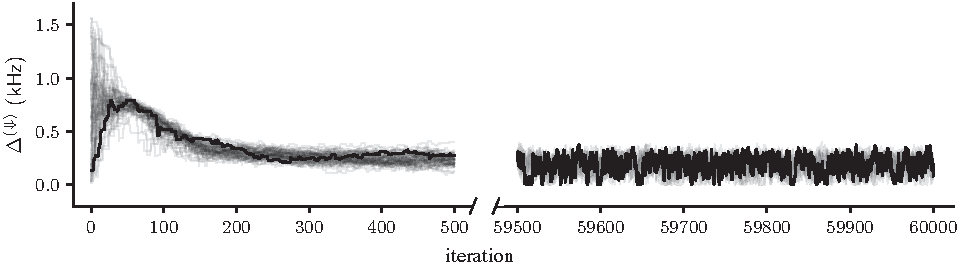
\includegraphics{chapter5/figures/chain.pdf}
    \caption[MCMC chain]{
    Example chain extracted from the ground state fit. The plot shows the evolution of one component of the walker ($\Delta^{(\Downarrow)}$) as a function of the iteration step for the first and last 500 steps. One arbitrary chain has been highlighted.}
    \labfig{chain}
\end{figure*}

where $z$ is the stretch factor that is sampled from a bounded distribution. If $z=1$ the point does not move; if $z>1$ the walker moves away from its pair, and if $z<1$ the walker moves toward its pair. Finally, the new position is accepted with probability $\alpha$, given by

\begin{equation}
    \alpha = \min\left(1, z^{d-1} \frac{\mathcal{L}(x_i')}{\mathcal{L}(x_i)}\right),
\end{equation}

where $\mathcal{L}$ is the logarithmic likelihood defined in \refsec{final_hamiltonian_fit}. This is repeated for all walkers and then iterated for a predefined number of steps. Convergence is not checked during the run and must be evaluated afterwards.


\section{Ground and excited fits}

Here we discuss the results of the fits performed in \refsec{final_hamiltonian_fit}. The algorithms were run with 64 walkers and 60000 iterations. An example chain is plotted in \reffig{chain} for the first and last 500 iterations. Two different behaviors can be observed. During the first 500 steps the parameter has still not converged and has a freer evolution. During the last 500 steps the chain has converged and the MCMC algorithm is exploring the parameter range where the logarithmic likelihood is maximized. To check for convergence, we perform this visual inspection after every fit.

\begin{figure*}[b!]
    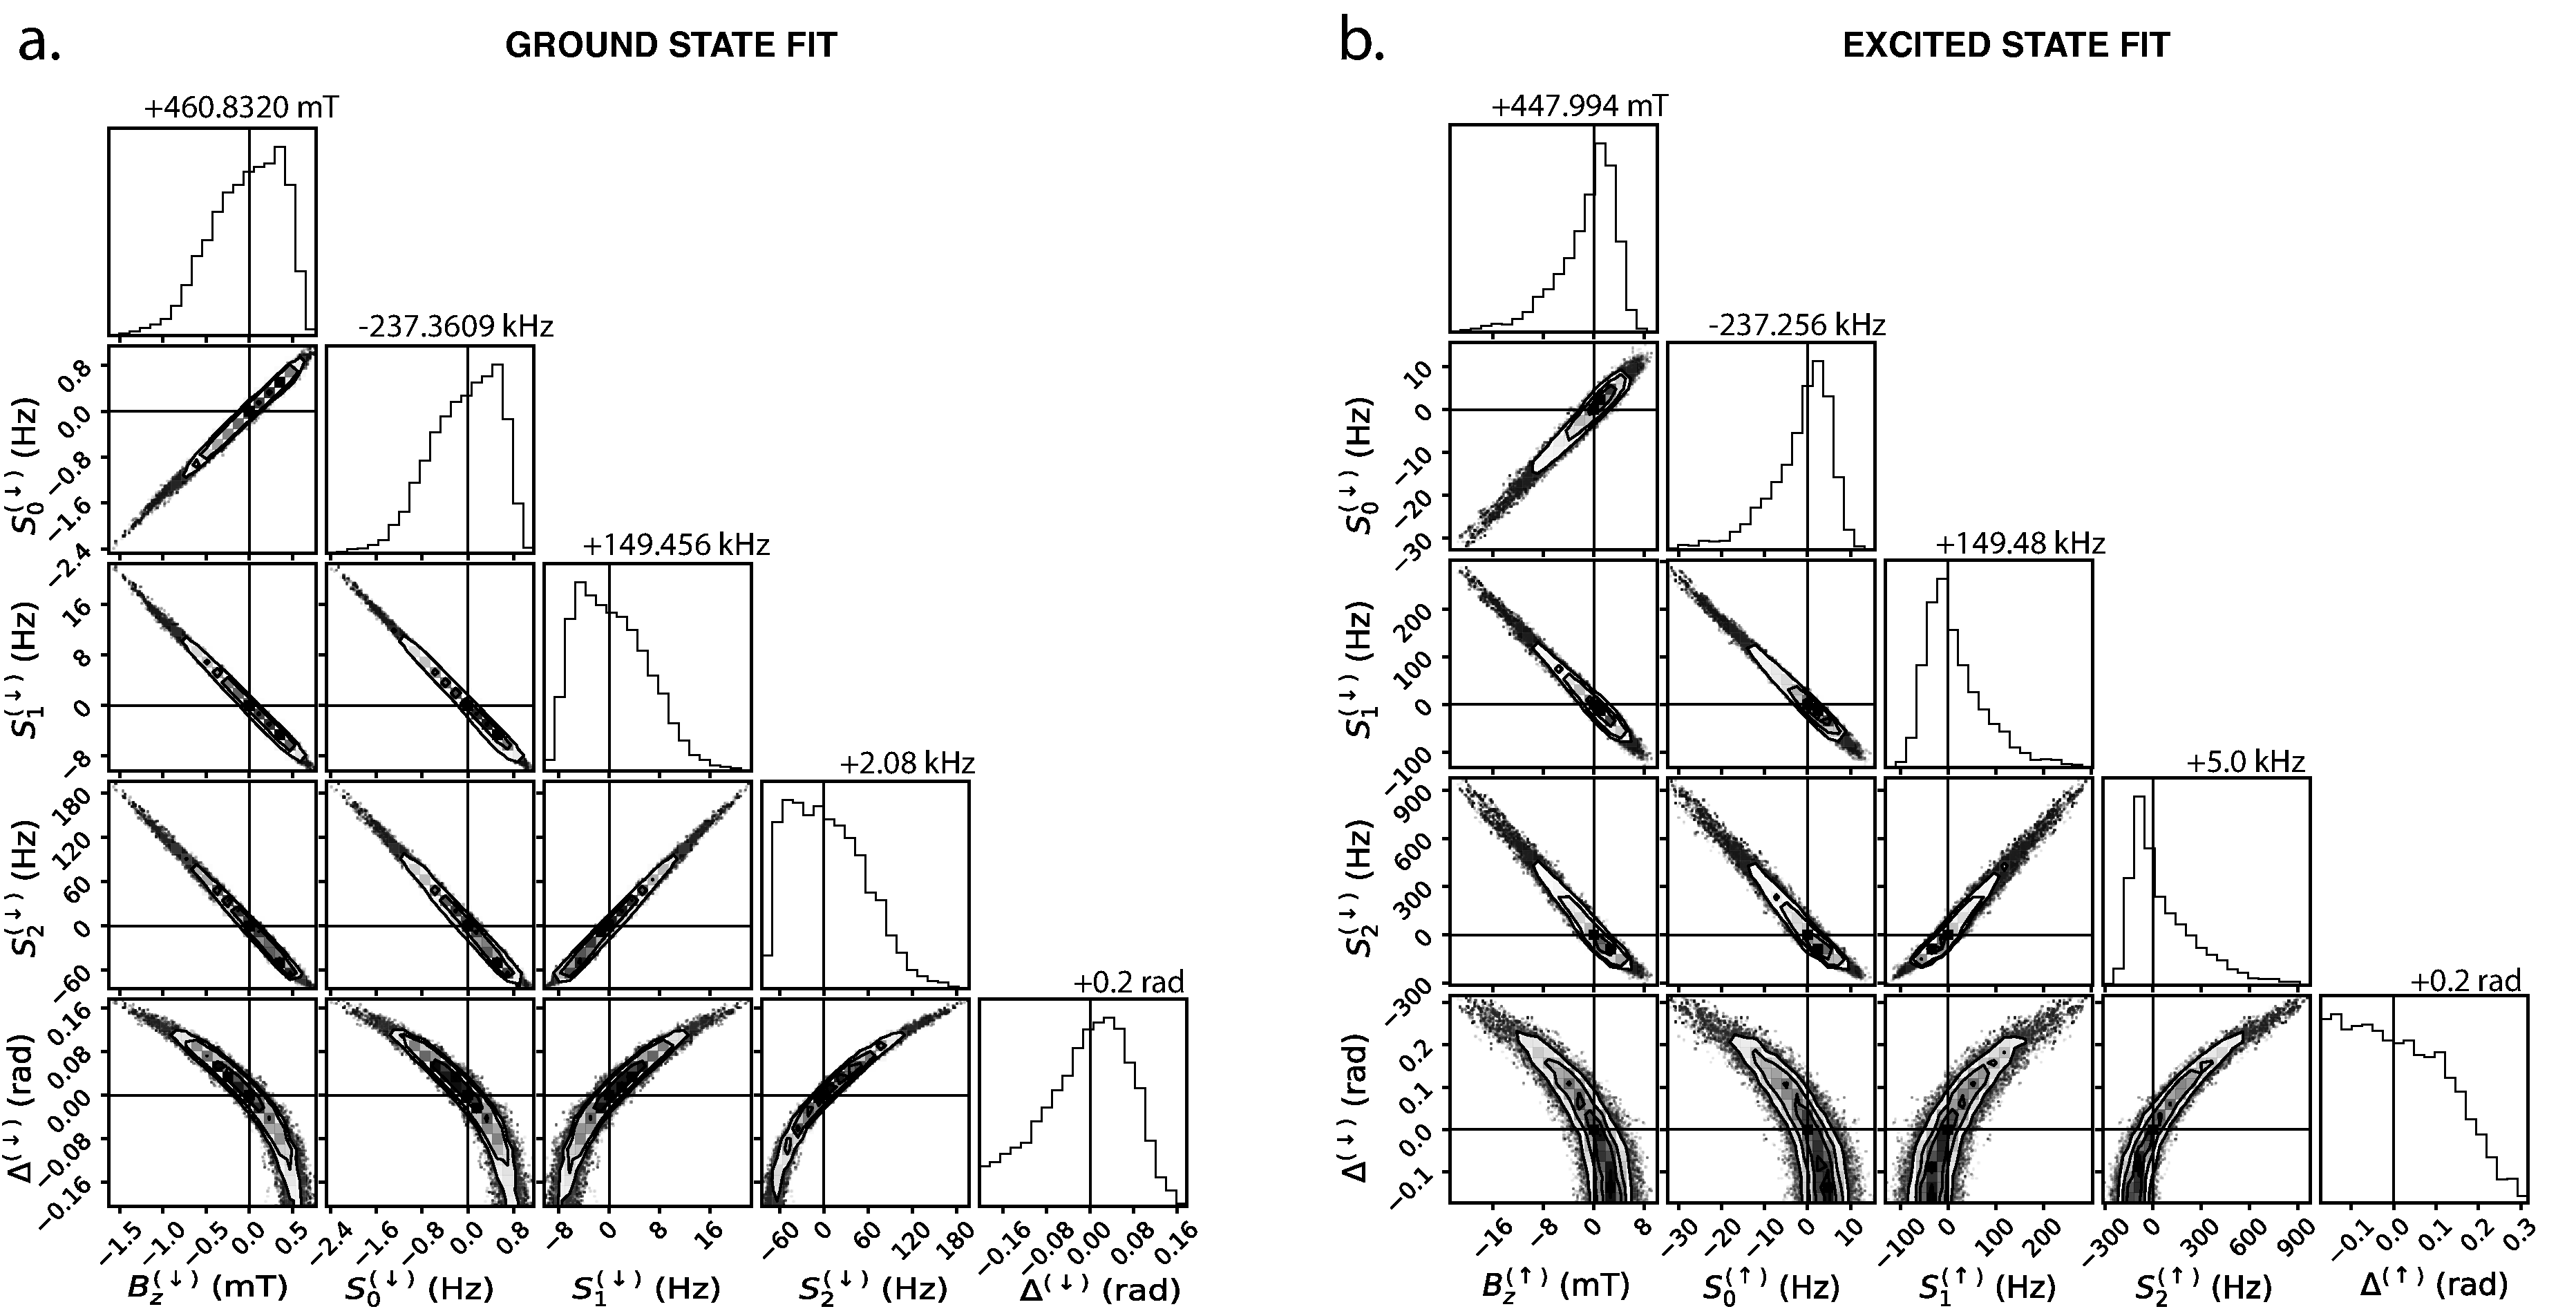
\includegraphics{chapter5/figures/corner_plot_dual.pdf}
    \caption[Corner plots of the separate Hamiltonian fits]{Separate Corner plots and chain trace. 
    \textbf{a \& b.} Corner plot of the posterior distributions of the MCMC fit in the ground and excited state (left and right resp.). Diagonal plots convey the one-dimensional distribution of the samples and off-diagonal plots the two-dimensional projection between two parameters. Vertical lines show the median value of the parameters, which we take as the result of the fit.}
    \labfig{corner_plot_dual}
\end{figure*}

In addition, we estimate the integrated autocorrelation time for each parameter to ensure that the number of effectively independent samples is sufficient. Since the chain length (60000) is at least 50 times larger than the autocorrelation time for all parameters (approximately 200 iterations), we conclude that we have obtained a large effective sample size.

We use the last 5000 iterations of the algorithm to obtain the final result, which is presented in the form of a corner plot~\sidecite{foreman-mackey_cornerpy_2016} in panels a and b of \reffig{corner_plot_dual} for the ground- and excited-state fits. The diagonal panels show the distribution of the individual parameters. The off-diagonal panels show the two-dimensional (2D) distributions as well as iso-probability bars. We take the final result of the fit as the median value of the distribution (shown as a cross) and the uncertainty as the standard deviation.

We note that the parameters show strong correlations, both linear and non-linear. These correlations mostly disappear when performing the fit with the full dataset, as shown in the next section. In addition, the distributions for $\Delta^{(m_S)}$ are cut at $\Delta^{(m_S)}=0$. This originates from the priors of the fit, where we limit $0<\Delta^{(m_S)}<\pi/2$ due to the periodic degeneracy of the variable. The large uncertainty of the parameter results in overlapping with the distribution of the next period, which is visualized as a flat region on the posterior distribution.

\section{Full Hamiltonian fit}

\begin{figure*}[b!]
    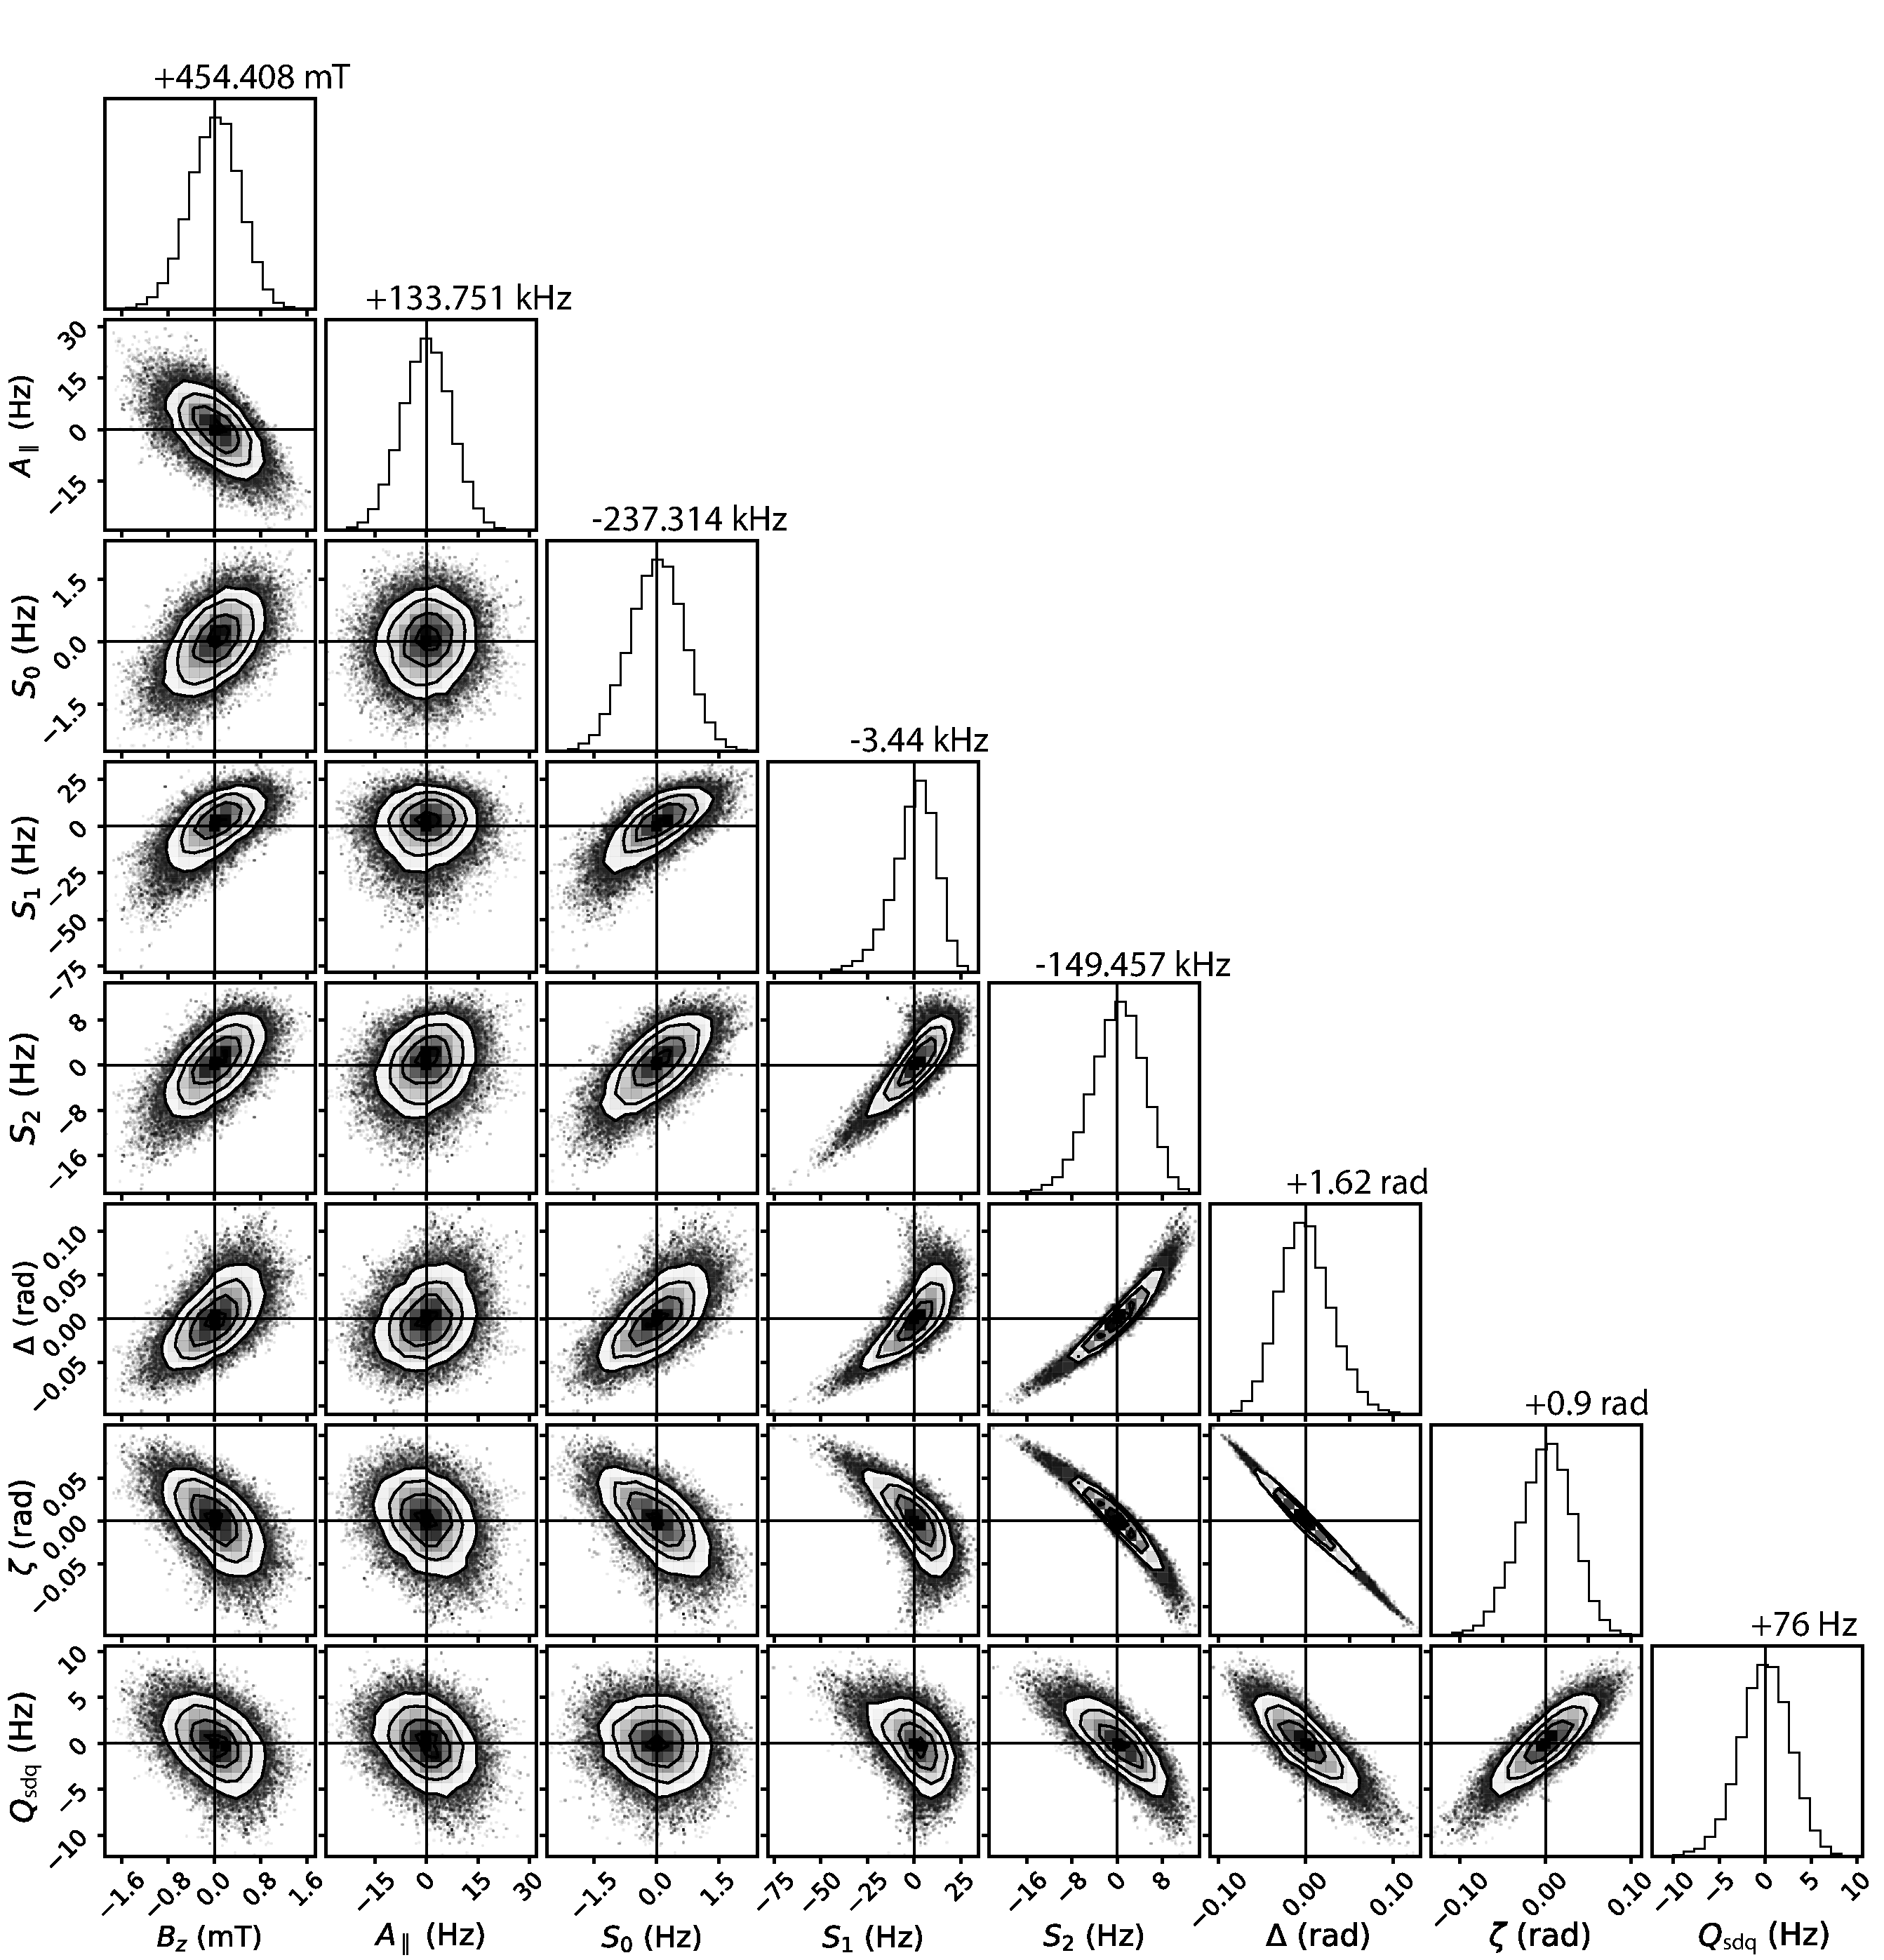
\includegraphics{chapter5/figures/corner_plot.pdf}
    \caption[Corner plot of the full Hamiltonian fit]{Corner plots of the posterior distributions of the full Hamiltonian fit. Diagonal plots convey the one-dimensional distribution of the samples and off-diagonal plots the two-dimensional projection between two parameters. Vertical lines show the median value of the parameters, which we take as the result of the fit.}
    \labfig{corner_plot}
\end{figure*}

The posterior distribution for the full Hamiltonian fit described in \refsec{final_hamiltonian_fit} is shown in \reffig{corner_plot}. Compared to the distributions of the previous figure, the correlations are mostly suppressed.

To account for the 9~kHz uncertainty in the measurement of $A_\perp$, we repeat the fit 400 times while sampling the value of $A_\perp$ from a Gaussian distribution with a standard deviation of 9~kHz. Each fit yields a median and standard deviation for the parameters. The final value of the parameter is obtained by taking the median of all 400 fit results. The final uncertainty is obtained by adding the standard deviation of all 400 fit results to the mean standard deviation of the posterior distributions. 

